%%% Preamble
\documentclass{report}

\usepackage[utf8]{inputenc}
\usepackage[T1]{fontenc}
\usepackage{fourier}
\usepackage[french]{babel}
\usepackage[protrusion=true,expansion=true]{microtype}	
\usepackage{amsmath,amsfonts,amsthm} % Math packages
\usepackage[pdftex]{graphicx}	
\usepackage{url}
\usepackage{pdfpages}
\usepackage{todonotes}
\usepackage[a4paper, body={16cm,26cm}]{geometry}
\usepackage{float}
\usepackage{framed}
\usepackage[toc,page]{appendix} 
\usepackage{multicol}
\usepackage{colortbl}
\usepackage{epstopdf}
\usepackage{adjustbox}

%%% Custom sectioning
\usepackage{sectsty}
\allsectionsfont{  \normalfont\scshape}
%\allsectionsfont{\centering \normalfont\scshape}

%%% Custom headers/footers (fancyhdr package)
\usepackage{fancyhdr}
\pagestyle{fancyplain}
\fancyhead{}								% No page header
\fancyfoot[L]{}							% Empty 
\fancyfoot[C]{}							% Empty
\fancyfoot[R]{\thepage}					% Pagenumbering
\renewcommand{\headrulewidth}{0pt}		% Remove header underlines
\renewcommand{\footrulewidth}{0pt}		% Remove footer underlines
\setlength{\headheight}{13.6pt}


%%% Equation and float numbering
\numberwithin{equation}{section}		% Equationnumbering: section.eq#
\numberwithin{figure}{section}		% Figurenumbering: section.fig#
\numberwithin{table}{section}		% Tablenumbering: section.tab#


%%% Define new commands
\newcommand{\horrule}[1]{\rule{\linewidth}{#1}} 	% Horizontal rule
\renewcommand{\bf}[1]{\textbf{#1}}
\renewcommand{\it}[1]{\textit{#1}}
\newcommand{\bfit}[1]{\textbf{\textit{#1}}}
\renewcommand{\sc}[1]{\textsc{#1}}

\newcommand{\Todo}[1]{\todo[inline]{#1}}
\renewcommand{\thesection}{\thepart .\arabic{section}}

\usepackage{tocloft}
\cftsetindents{chapter}{0em}{1em}
\cftsetindents{section}{1.5em}{2.5em}
\makeatletter
\def\l@figure{\@dottedtocline{1}{1.5em}{4em}}
\makeatother

\usepackage{bookmark}
%\usepackage[hidelinks]{hyperref}
\usepackage{cases}
\usepackage{color}
\usepackage{xcolor}
\usepackage{relsize}
\usepackage{caption}
\colorlet{shadecolor}{black!10}

\delimitershortfall-1sp
\newcommand\abs[1]{\left|#1\right|}


\usepackage{tikz, pgfplots}


%}}}
%{{{ --- pgfplots ---------------------

%{{{ Colors

% TolColors from http://www.r-bloggers.com/the-paul-tol-21-color-salute/
\definecolor{TolColor1}{HTML}{332288}   % dark purple
\definecolor{TolColor2}{HTML}{6699CC}   % dark blue
\definecolor{TolColor3}{HTML}{88CCEE}   % light blue
\definecolor{TolColor4}{HTML}{44AA99}   % light green
\definecolor{TolColor5}{HTML}{117733}   % dark green
\definecolor{TolColor6}{HTML}{999933}   % dark brown
\definecolor{TolColor7}{HTML}{DDCC77}   % light brown
\definecolor{TolColor8}{HTML}{661100}   % dark red
\definecolor{TolColor9}{HTML}{CC6677}   % light red
\definecolor{TolColor10}{HTML}{AA4466}  % light pink
\definecolor{TolColor11}{HTML}{882255}  % dark pink
\definecolor{TolColor12}{HTML}{AA4499}  % light purple

%}}}
%{{{ Color cycles

\pgfplotscreateplotcyclelist{mbarplot cycle}{%
  {draw=TolColor2, fill=TolColor2!70},
  {draw=TolColor7, fill=TolColor7!70},
  {draw=TolColor4, fill=TolColor4!70},
  {draw=TolColor11, fill=TolColor11!70},
  {draw=TolColor1, fill=TolColor1!70},
  {draw=TolColor8, fill=TolColor8!70},
  {draw=TolColor6, fill=TolColor6!70},
  {draw=TolColor9, fill=TolColor9!70},
  {draw=TolColor10, fill=TolColor10!70},
  {draw=TolColor12, fill=TolColor12!70},
  {draw=TolColor3, fill=TolColor3!70},
  {draw=TolColor5, fill=TolColor5!70},
}

\pgfplotscreateplotcyclelist{mlineplot cycle}{%
  {TolColor2, mark=*, mark size=1.5pt},
  {TolColor7, mark=square*, mark size=1.3pt},
  {TolColor4, mark=triangle*, mark size=1.5pt},
  {TolColor6, mark=diamond*, mark size=1.5pt},
}


\pgfplotsset{
  compat=1.9,
  mbaseplot/.style={
    legend style={
      draw=none,
      fill=none,
      cells={anchor=west},
    },
    x tick label style={
      font=\footnotesize
    },
    y tick label style={
      font=\footnotesize
    },
    legend style={
      font=\footnotesize
    },
    major grid style={
      dotted,
    },
    axis x line*=bottom,
  },
  mlineplot/.style={
    mbaseplot,
    xmajorgrids=true,
    ymajorgrids=true,
    major grid style={dotted},
    axis x line=bottom,
    axis y line=left,
    legend style={
      cells={anchor=west},
      draw=none
    },
    cycle list name=mlineplot cycle,
  },
  mbarplot base/.style={
    mbaseplot,
    bar width=6pt,
    axis y line*=none,
  },
  mbarplot/.style={
    mbarplot base,
    ybar,
    xmajorgrids=false,
    ymajorgrids=true,
    area legend,
    legend image code/.code={%
      \draw[#1] (0cm,-0.1cm) rectangle (0.15cm,0.1cm);
    },
    cycle list name=mbarplot cycle,
  },
  horizontal mbarplot/.style={
    mbarplot base,
    xmajorgrids=true,
    ymajorgrids=false,
    xbar stacked,
    area legend,
    legend image code/.code={%
      \draw[#1] (0cm,-0.1cm) rectangle (0.15cm,0.1cm);
    },
    cycle list name=mbarplot cycle,
  },
  disable thousands separator/.style={
    /pgf/number format/.cd,
      1000 sep={}
  },
}


%%  ========   IMPORTANT ========
%% Spécifier ici les variables pour le document
\newcommand{\mainTitle}{\'Etude préalable - SPIE}
\newcommand{\secondTitle}{Spécification du SI cible}
\newcommand{\documentRef}{DEB-SSIC/4401/1}
\newcommand{\auteurs}{
Lisa \textsc{Courant} \\
Estelle \textsc{Lepeigneux} \\
Pierre \textsc{Jarsaillon} \\
Hugues \textsc{Verlin} \\
}
\newcommand{\chefDeProjet}{Paul \textsc{Dautry}}
\newcommand{\responsableQualite}{Antoine \textsc{Chabert}}

%%% Begin document
\begin{document}
%----------------------------------------------------------------------------------------
%	PACKAGES
%----------------------------------------------------------------------------------------

\documentclass[12pt]{article}
\usepackage[a4paper]{geometry}
\geometry{verbose,tmargin=1in,bmargin=0in,lmargin=1in,rmargin=1in}
\usepackage[utf8]{inputenc}
\usepackage[francais]{babel}
\usepackage[T1]{fontenc}

\usepackage{graphicx}
\begin{document}

\begin{titlepage}

\newcommand{\HRule}{\rule{\linewidth}{0.5mm}} % horizontal lines

\center % Center everything
 
%----------------------------------------------------------------------------------------
%	HEADING SECTIONS
%----------------------------------------------------------------------------------------

\vspace*{1cm}

\textsc{\LARGE INSA de LYON}\\[1.5cm] 
\textsc{\Large D\'epartement Informatique}\\[0.5cm] 
\textsc{\large Projet Longue Durée}\\[0.5cm] % 

%----------------------------------------------------------------------------------------
%	TITLE SECTION
%----------------------------------------------------------------------------------------

\HRule \\[0.4cm]
{ \huge \bfseries Compte Rendu}\\[0.1cm]
{\large \bfseries - Gestion des contacts commerciaux d'une banque -} 
\HRule \\[1.5cm]
 
%----------------------------------------------------------------------------------------
%	DATE SECTION
%----------------------------------------------------------------------------------------

{\large \today}\\[2cm] % 
 
%----------------------------------------------------------------------------------------
%	AUTHOR SECTION
%----------------------------------------------------------------------------------------

\begin{minipage}{0.4\textwidth}
\begin{center} \large
\emph{Auteurs} \\
Lisa \textsc{Courant} \\
Estelle \textsc{Lepeigneux} \\
Pierre \textsc{Jarsaillon} \\
Hugues \textsc{Verlin} \\
\end{center}
\end{minipage}
~
\begin{minipage}{0.4\textwidth}
\begin{center} \large
\emph{Chef de projet} \\
Paul \textsc{Dautry}
\end{center}
\begin{center} \large
\emph{Responsable Qualité} \\
Antoine \textsc{Chabert}
\end{center}
\end{minipage}\\[5cm]

H4401\\[2cm]

%----------------------------------------------------------------------------------------
%	LOGO SECTION
%----------------------------------------------------------------------------------------

\includegraphics[scale=0.3]{figures/logo.png}
%----------------------------------------------------------------------------------------

\vfill % Fill the rest of the page with whitespace

\end{titlepage}
\end{document}


%% Commenter les deux lignes suivantes pour le document final
%\listoftodos
%\newpage

%% Table de matière / figures / tableaux
\tableofcontents
\listoffigures
\listoftables
\newpage

%% Faire une nouvelle partie :
\part{Thèmes des progrès fonctionnels}
\setcounter{section}{0}

\section{Suivi de l’activité et mise en place d’un tableau de bord}

Un autre axe intéressant à explorer peut être de mettre en place des indicateurs de performance. 
Ce type de tableau de bord permet à SPIE de pouvoir visualiser simplement l’évolution des performances de l’entreprise. De plus, si ce système est mis en place assez tôt, il permettra d’avoir un retour sur les impacts de la mise en place des autres propositions ici présentes. \\

Ce tableau de bord pourrait regrouper les informations suivantes : \\
    
Indicateurs de type organisationnel : il s’agit ici de relever le nombre d’interventions, le profil type des intervenants en fonction des situations, etc.\\
Indicateurs de type techniques : il s’agit ici d’indiquer la nature des travaux, le temps moyen passés sur un contrat, ou encore les moyens mobilisés\dots \\
Indicateurs économiques : on s’intéresse là à observer la marge, ou encore le rendements des contrats\dots \\

Toujours dans l’idée d’améliorer le suivi et afin de pouvoir estimer plus précisément les recettes de prestations, nous avons décidé de standardiser la phase d’achat des pièces de maintenance lors du lancement de prestation de services et de travaux. Ainsi, en estimant les pièces de rechange nécessaires après l’état des lieux du site, on peut vérifier leur disponibilité dans le stock, puis le réapprovisionner en amont de la réalisation des prestations.

\section{Évolution et mise en place de la mobilité}

Afin d’améliorer l’efficacité de ses processus et l’accès au reporting, il peut être intéressant pour SPIE de doter ses collaborateurs d’appareils mobiles ainsi que d’applications dédiées à ses besoins. En effet, la mise en place d’une application mobile pour les techniciens réalisant les différentes tâches de maintenance pourra favoriser la rédaction de retours d’expériences, directement à partir de leur terminal mobile. L’application, communiquant avec le système d’information de SPIE Sud-Est, permettra ainsi d’alimenter la base de connaissances de SPIE et permettant, à termes, d’exploiter les retours d’expérience afin d’améliorer la qualité des services fournis par SPIE. En effet, le technicien pouvant remplir sa fiche de retour d’expérience directement après son intervention, le risque d’omission est diminué, les événements et problématiques rencontrés étant encore récents. De plus, en cas de retour client, positif ou négatif, suite à l’intervention, le technicien peut adapter son retour d’expérience en fonction des impressions recueillies sur le terrain, augmentant davantage sa mobilité. \\

La mise en place d’une mobilité pour les techniciens a également pour avantage de leur permettre d’accéder aux différentes informations dont ils ont besoin sur le terrain, leur évitant ainsi d’accumuler des documents, au risque d’oublier, voir perdre, des informations importantes. Le gain de temps peut ainsi mettre mis à profit, permettant au technicien de se concentrer sur sa tâche, rehaussant de nouveau la qualité des services de maintenance et rejoignant un des objectifs principaux de SPIE Sud-Est, à savoir l’amélioration de la qualité des prestations. \\

De plus, l’application mobile mise en place pourra être modulaire, permettant ainsi de développer progressivement les modules correspondant aux besoins des différents acteurs de la société. Il faut également noter que l’utilisation d’une application mobile par les acteurs d’une société permet de renforcer l’image de celle-ci. En effet, cela véhicule une image interne et externe de modernité et de veille technologique.\\

La mise en place d’une application mobile au sein de SPIE Sud-Est, à destination dans un premier temps aux techniciens réalisant les interventions de maintenant, permettrait donc d’améliorer la communication avec le système d’information lors des interventions, mais également d’améliorer l’image de la société.\\

\section{Amélioration de la gestion des risques}

Actuellement, l’analyse des risques est effectuée ponctuellement, sans réel suivi sur le long terme. Il serait donc intéressant de mettre en oeuvre une gestion des risques plus poussée et plus régulière, qui interviendrait tout au long de la réalisation du contrat. Pour cela, il faudrait mettre en place un nouvel indicateur, l’indice de niveau de sécurité, qui interviendrait non seulement à des moments clés de la réalisation, mais également tout au long du processus. Ainsi, à chaque réalisation de prestation, une mise à jour des risques et, à fortiori, des indicateurs associés, sera à prévoir, après chaque revue périodique du contrat. De plus, un bilan des risques sera réalisé lors de la solde du contrat, afin de faire un point sur le déroulement de celui-ci. \\

Cette amélioration s’inscrit dans une optique de Business Intelligence, ou BI, en combinaison avec une base de connaissance. En effet, l’accumulation des données concernant la gestion des risques, grâce à une surveillance accrue, permettra de de tirer parti des différentes informations accumulées au fil des expériences. Tirer parti des éventuels problèmes rencontrés permettra ainsi de mieux prévoir les éventuels risques pouvant intervenir par la suite et, de fait, garantir une meilleure qualité de service. En effet, garder une trace des problèmes ayant survenus permet de proposer aux acteurs de la société les méthodes de résolution qui ont été mises en oeuvres précédemment. Cela permettra également de pouvoir mieux juger en amont les offres, lors des phases de négociation client. Ces dernières pourront ainsi être éventuellement jugées comme étant à risque potentiel et ainsi mettre en place une surveillance accrue du déroulement du contrat, si celui-ci est tout de même accepté. \\

La mise en place d’une gestion améliorée des risques permettrait donc à la fois d’augmenter la qualité des services proposés par SPIE Sud-Est, grâce à une augmentation de la satisfaction client, mais apporterait également une situation de confort aux acteurs de la société. En effet, la confrontation aux situations à risque étant partiellement prise en charge par cette nouvelle gestion des risques, les employés de SPIE Sud-Est sont alors soumis à moins de stress, améliorant ainsi leurs conditions de travail et, de fait, leur capacité de travail.


\part{Thèmes des progrès techniques}
\setcounter{section}{0}

\section{Favoriser la migration vers un nouveau système d’information uniformisé}

Comme mentionné au préalable dans la section Étude de l’existant, le système d’information actuel de SPIE est constitué de nombreuses applications différentes, s’intégrant plus ou moins difficilement à leur ERP actuel, PeopleSoft. Cependant, cette organisation induit des flux de données pouvant être hétérogènes car non normalisés, voir redondant. Cela provoque des difficultés de maintenance, avec des risques d’erreurs sur les données circulant sur le système d’information, tout en augmentant les coûts de maintenance. \\

L’étude réalisée ayant pour objectif de dégager de nouvelles solutions afin d’améliorer les activités de maintenance de SPIE, il est important d’avoir un système d’information modulaire, apte à intégrer de nouvelles modifications. Cependant, le passage d’un système d’information à un autre ne peut se faire sans planification précise. En effet, le système d’information actuel est composé d’un ERP, qui en constitue une grande partie, complexifiant davantage l’éventuelle migration vers un nouveau système. Sans planification détaillée et progressive, la migration peut provoquer des pertes financières, voir des pertes de données, qui peuvent se révéler plus problématiques à long terme. A l’heure actuelle, où le numérique est omniprésent dans les sociétés, les données numériques s’accumulent à grande vitesse et deviennent de vraies richesses pour les entreprises, qui peuvent ensuite les exploiter pour dégager des axes de développement. \\

Un remplacement abrupt de l’ERP PeopleSoft est également déconseillé vis-à-vis des utilisateurs, qui devront être formés à l’utilisation d’une nouvelle application, de grande complexité en termes de fonctionnalités. Un axe d’amélioration pouvant être envisagé, est donc une migration très progressive et partielle du système d’information actuel de SPIE, vers un nouveau système d’information normalisé. Cela permettrait de former au fur et à mesure les utilisateurs, tout en recueillant leurs impressions sur leur nouvelle plate-forme de travail, afin d’adapter si besoin les paramètres et personnalisations des nouvelles applications. Ainsi, une mise en place d’une architecture ERP 2-tiers, permettant de faire fonctionner les deux ERP simultanément (PeopleSoft et l’ERP retenu par la suite de l’étude), est à envisager, tout en permettant de budgétiser dans le temps la migration.

\section{Mise en place d’une base de connaissances}

La centralisation et la gestion des connaissances est primordiale pour une entreprise telle que SPIE, de même que l’est la capacité à pouvoir avoir des retours sur les missions qu’effectuent les techniciens lors des opérations de maintenance. \\

Les phases de reporting ne doivent plus être négligées et doivent faire l’objet de processus soigneusement étudiés afin d’être le plus utiles possibles, afin de faire ensuite gagner du temps à l’entreprise. \\

Ainsi, dans un objectif d’amélioration continue de la qualité de travail de ses collaborateurs, il peut être proposé à SPIE de mettre en place des fonctions de recueils des retours de l’ensemble des personnes travaillant à SPIE, mais également de récupérer un retour de la part de ses clients. \\

Il serait alors intéressant de coupler cette base avec une solution de Business Intelligence afin d’analyser aux mieux les retours. \\

Afin d’intégrer cette idée dans les processus de SPIE, nous allons ajouter les liens avec la base de connaissances, c’est-à-dire aux moments où nous allons la mettre à jour et l’utiliser dans le cadre de la Business Intelligence. On peut aussi mettre en place l’envoi d’un questionnaire de satisfaction client après chaque intervention pour avoir un retour du client sur les prestations de l’entreprise et ainsi de pouvoir évaluer la qualité de cette dernière.


%% ANNEXES ---------------------------------------------------------------------------

\appendix
\chapter{Modèle Conceptuel de Données de la cible}

\begin{figure}[H]
    \label{fig-mcd-cible}
    \noindent\makebox[\textwidth]{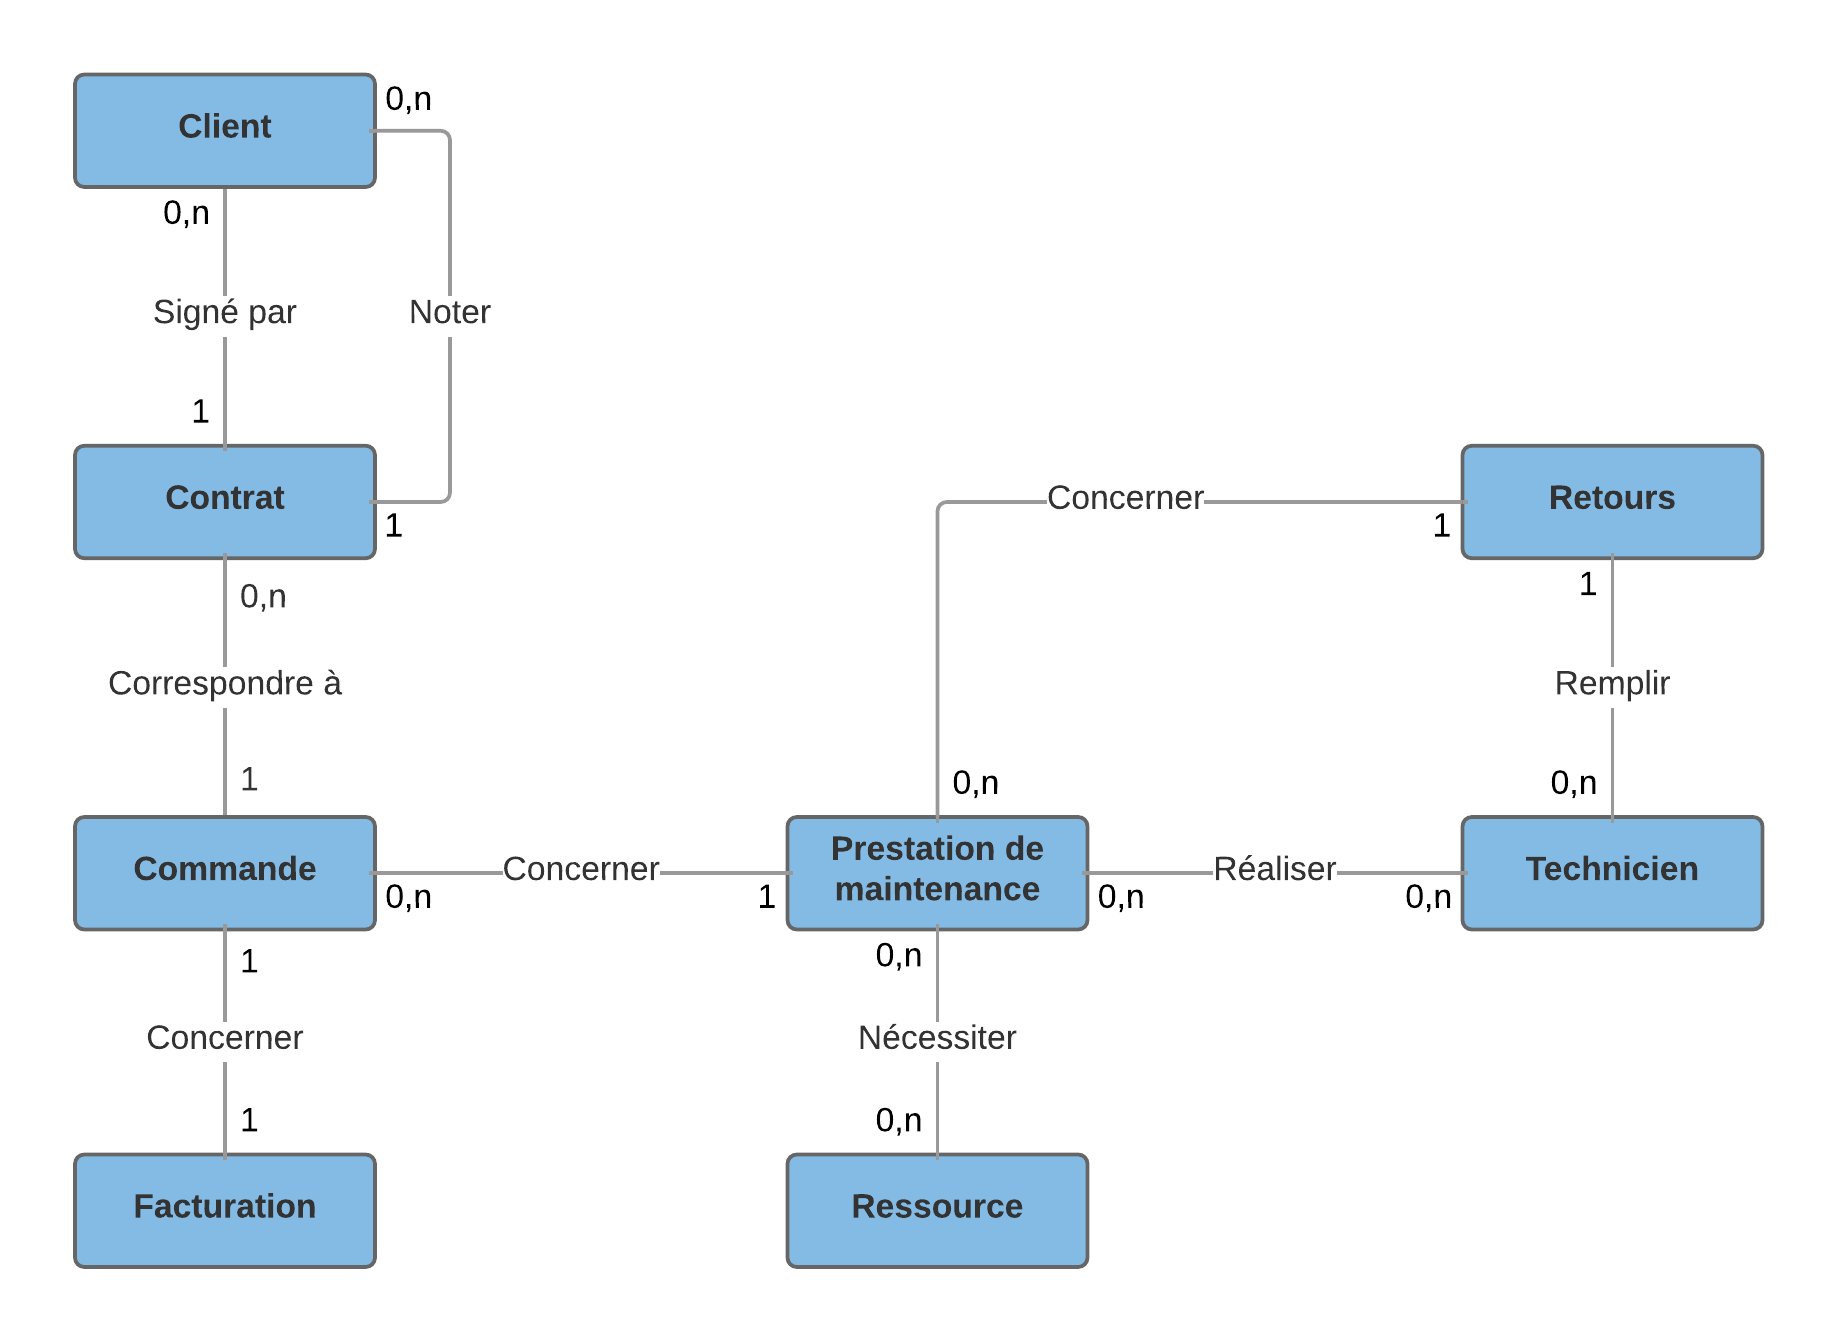
\includegraphics[width=10cm]{figures/mcd_cible.png}}
    \caption{Modèle conceptuel de données de la cible}
\end{figure}

\chapter{Modèle Organisationnel}

\begin{figure}[H]
    \label{fig-organisationnel}
    \noindent\makebox[\textwidth]{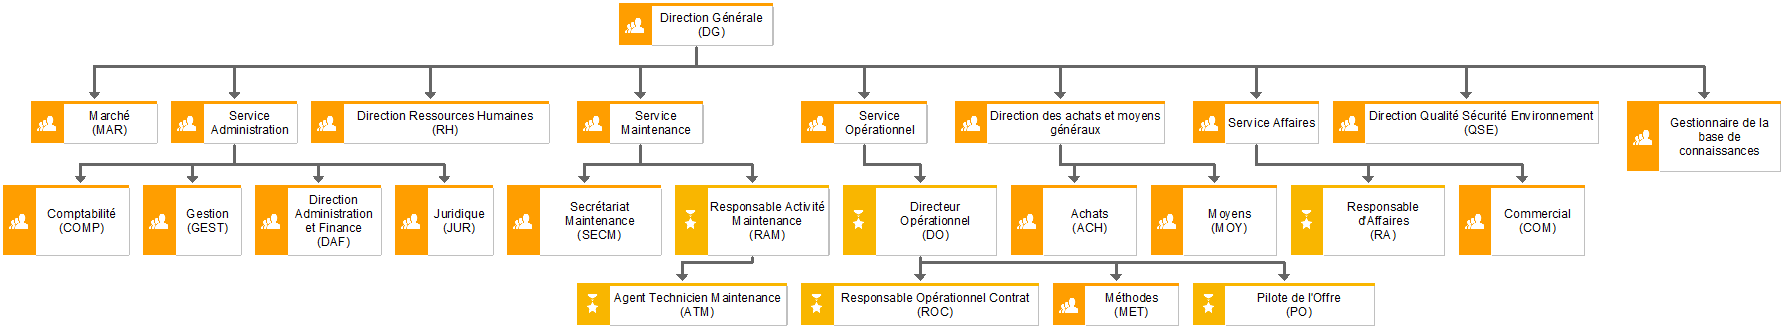
\includegraphics[width=20cm,angle=90]{figures/organisation_cible.png}}
    \caption{Modèle organisationnel}
\end{figure}

\chapter{Modèle ARIS de la cible}

\begin{figure}[H]
    \label{fig-commande-revue}
    \noindent\makebox[\textwidth]{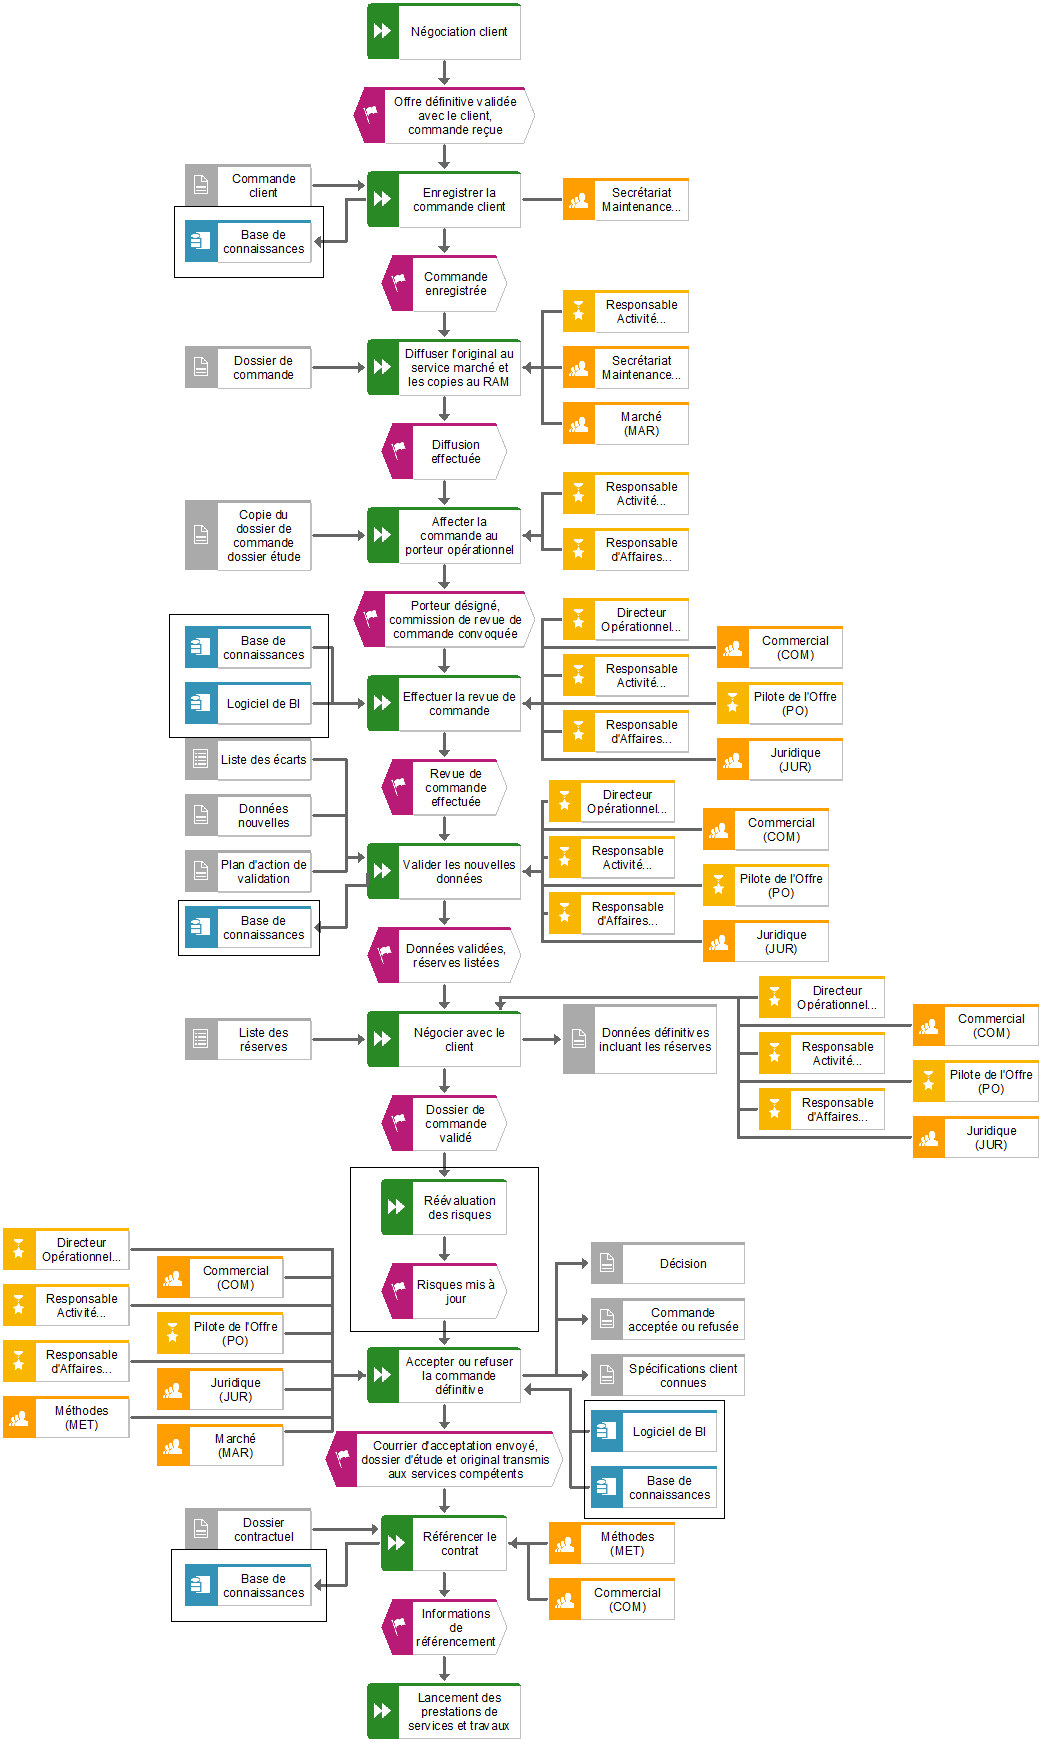
\includegraphics[width=10cm]{figures/aris/commande_revue_de_commande.png}}
    \caption{Commande et Revue de Commande}
\end{figure}

\begin{figure}[H]
    \label{fig-evol-contrat}
    \noindent\makebox[\textwidth]{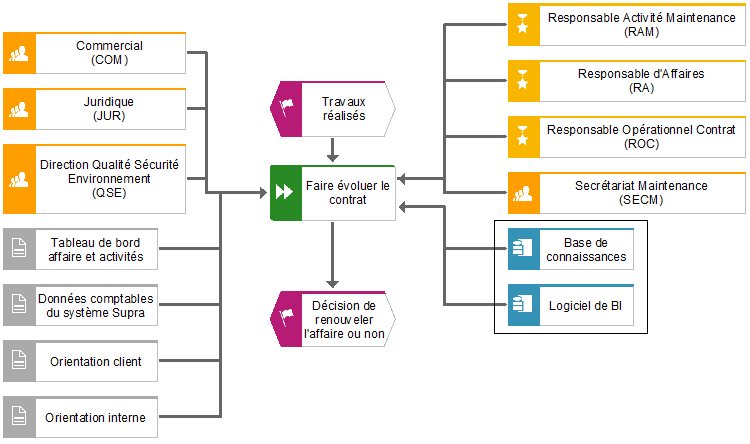
\includegraphics[width=10cm]{figures/aris/evolution_contrat.png}}
    \caption{Processus Evolution du Contrat}
\end{figure}

\begin{figure}[H]
    \label{fig-lancement}
    \noindent\makebox[\textwidth]{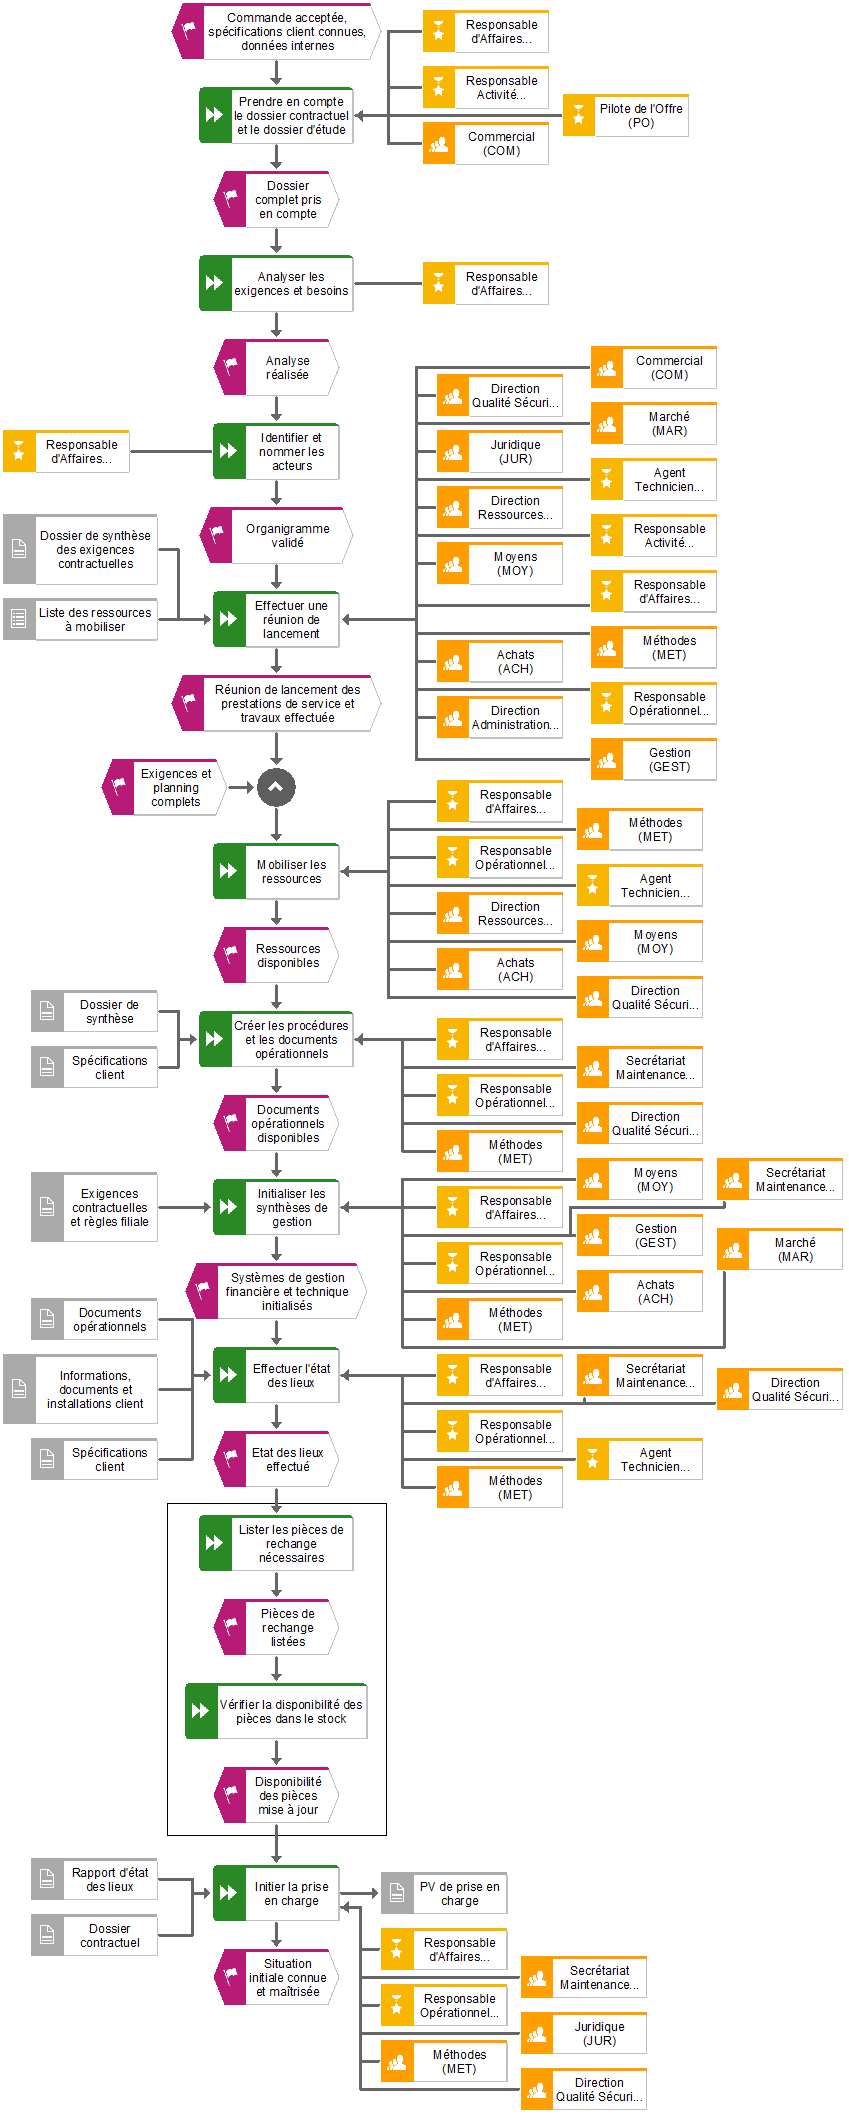
\includegraphics[width=10cm]{figures/aris/lancement_presatations_de_services_et_travaux_avec_roles.png}}
    \caption{Processus Lancement des Prestations de Services et Travaux avec rôles}
\end{figure}

\begin{figure}[H]
    \label{fig-offre-revue}
    \noindent\makebox[\textwidth]{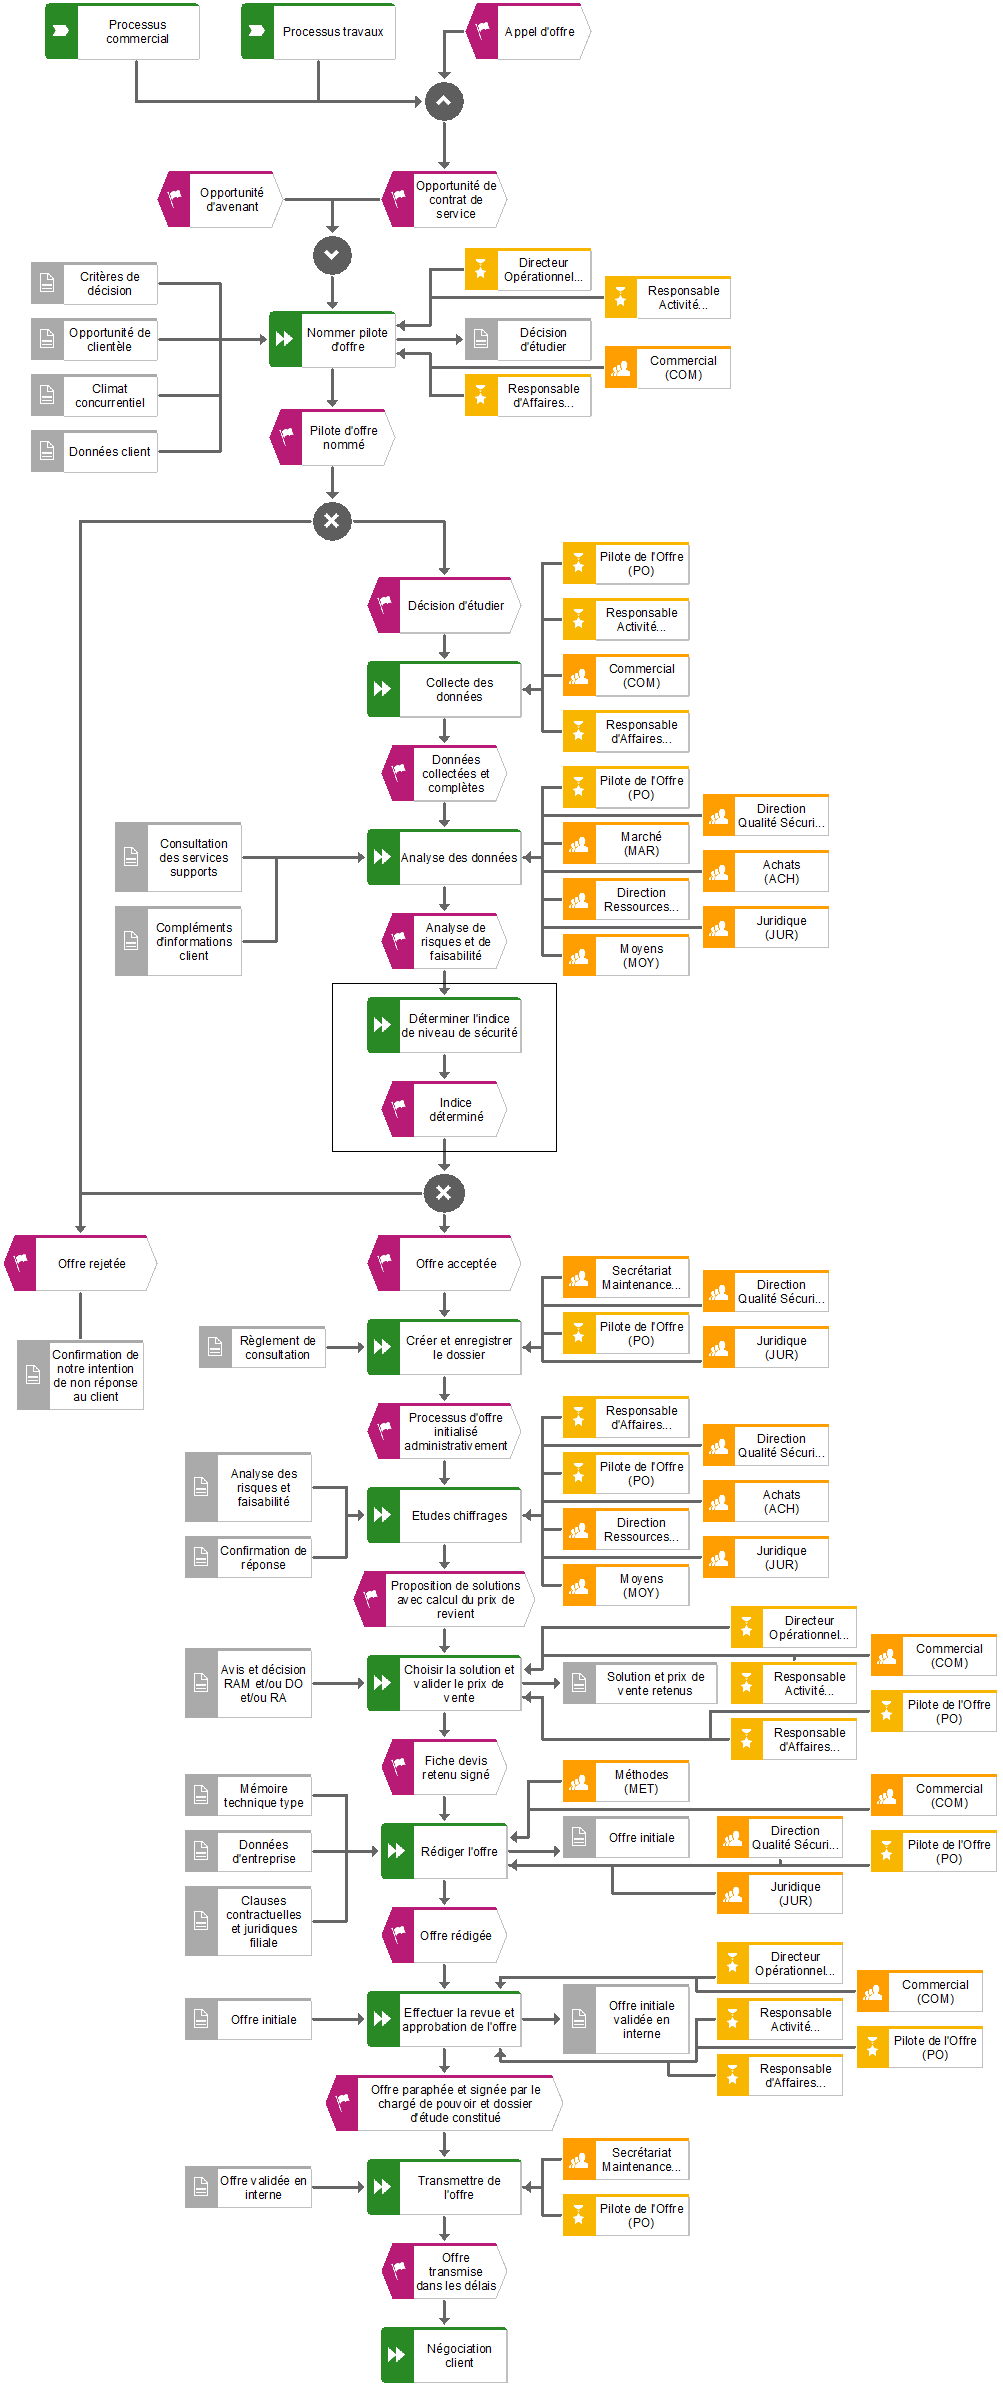
\includegraphics[width=10cm]{figures/aris/offre_revue_doffre.png}}
    \caption{Processus Offre et Revue d'Offre}
\end{figure}

\begin{figure}[H]
    \label{fig-real-prest}
    \noindent\makebox[\textwidth]{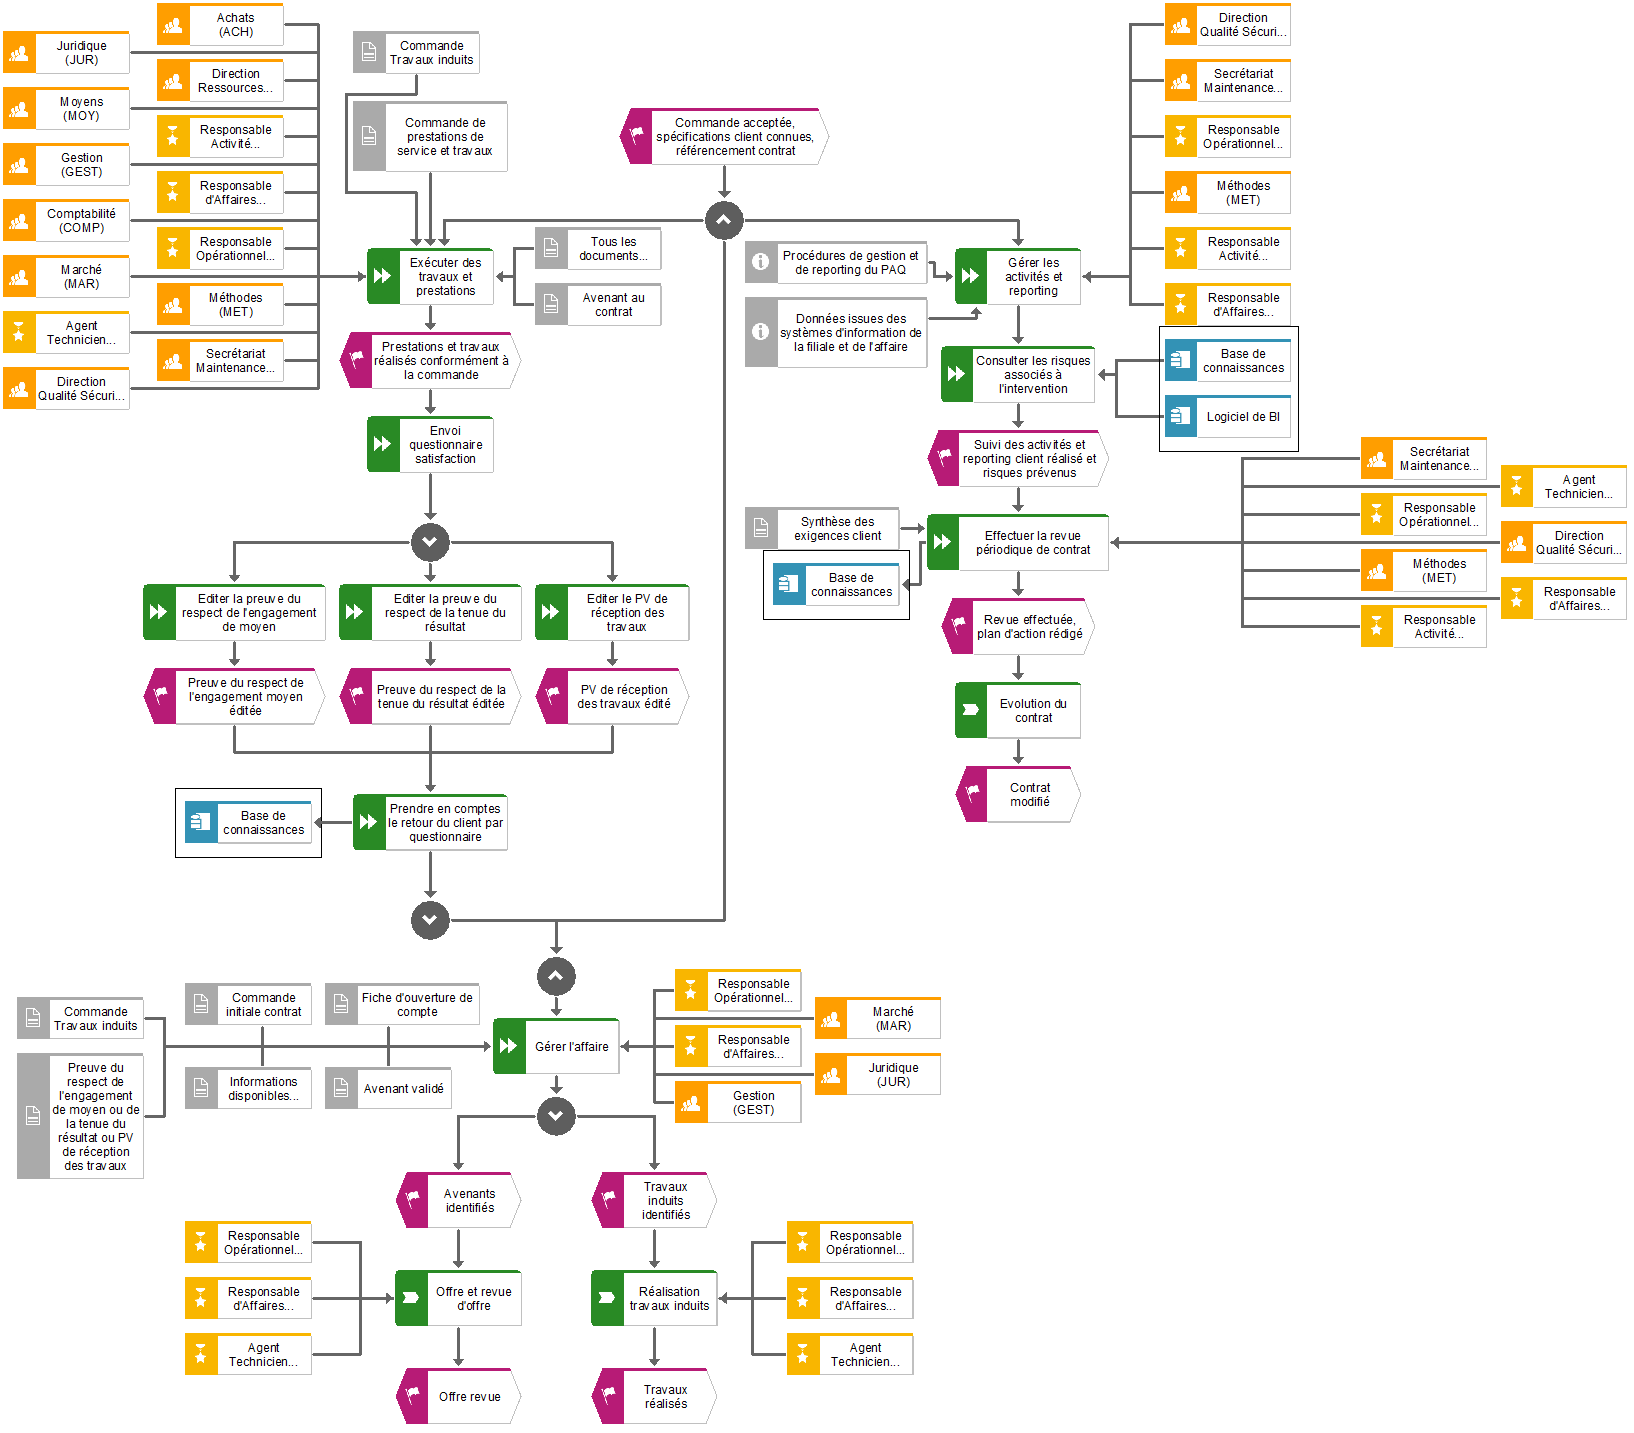
\includegraphics[width=14cm]{figures/aris/realisation_de_prestations_de_maintenance.png}}
    \caption{Processus Réalisation Prestations de Maintenance}
\end{figure}

\begin{figure}[H]
    \label{fig-solde-affaire}
    \noindent\makebox[\textwidth]{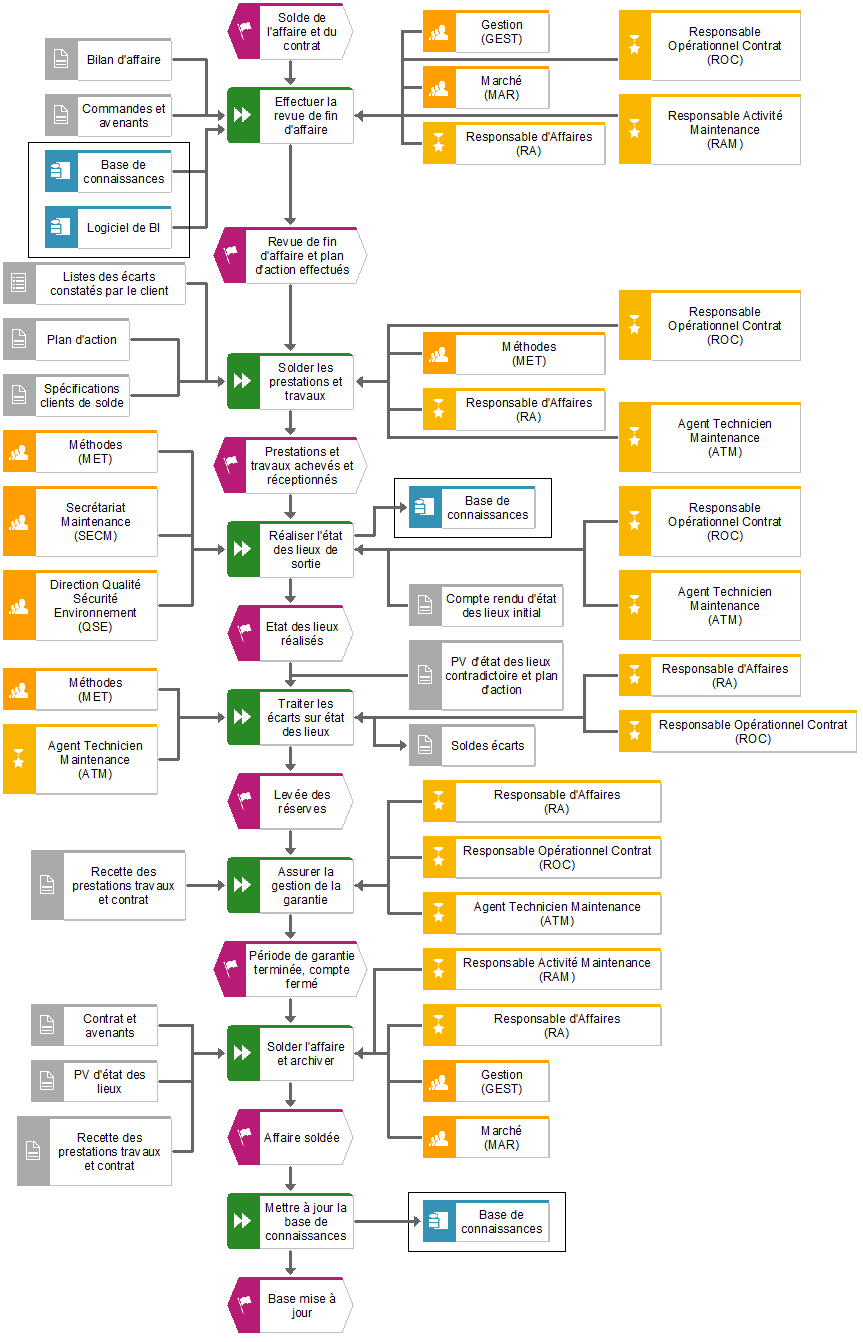
\includegraphics[width=12cm]{figures/aris/solde_de_laffaire_et_du_contrat.png}}
    \caption{Processus Solde de l'Affaire et du Contrat}
\end{figure}


\chapter{Matrice ARIS Fonction - Rôle}

\begin{figure}[H]
    \label{fig-matrice}
    \noindent\makebox[\textwidth]{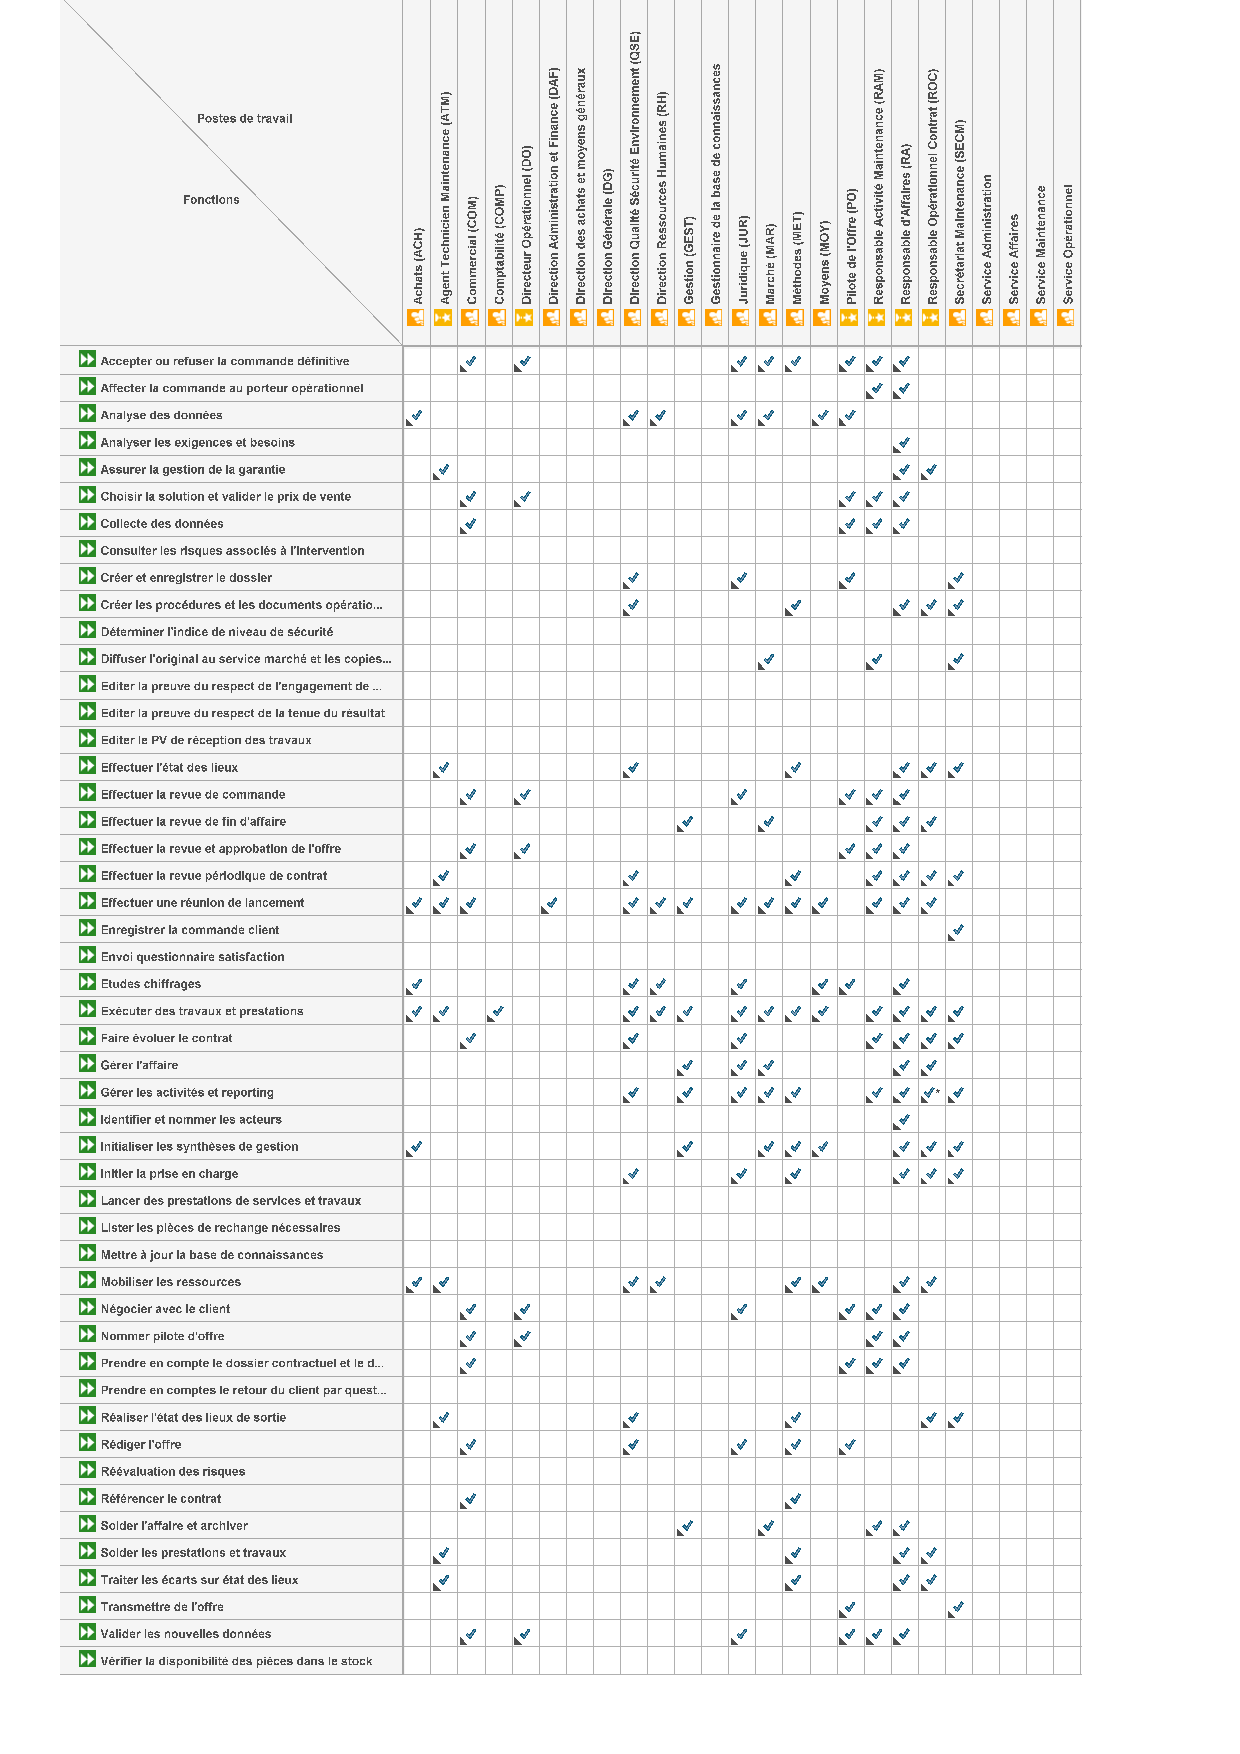
\includegraphics[width=14cm]{pdf_externes/matrice_cible.pdf}}
    \caption{Commande et Revue de Commande}
\end{figure}

%%% End document
\end{document}
